\section{Experimental Evaluation}

In this section, we present empirical and analytical evaluation of the performance and cost of \sysname under different workloads and scales. 
% \begin{itemize}
% \item What is performance and cost of 
% \end{itemize}

\noindent \textbf{Environment and Workloads:} All our empirical evaluation is conducted with the \sysname prototype on the Google Public Cloud, and with these open-source scientific applications:
\begin{description}
\item[NC.] Ions in Nanoconfiment~\cite{} configured with OpenMP and MPI. 
\item[Shapes.] 
\item[Lulesh.] Popular hydrodynamics application with default parameters. 
\end{description}

All applications use OpenMPI and 64-bit Ubuntu 18.04 as the base OS.
All the Google Cloud VMs are x86-64 Intel Broadwell, with different number of cores and memory sizes depending on the VM size selected. 



\subsection{SciSpot Performance and Cost}

\begin{figure}
  \centering
  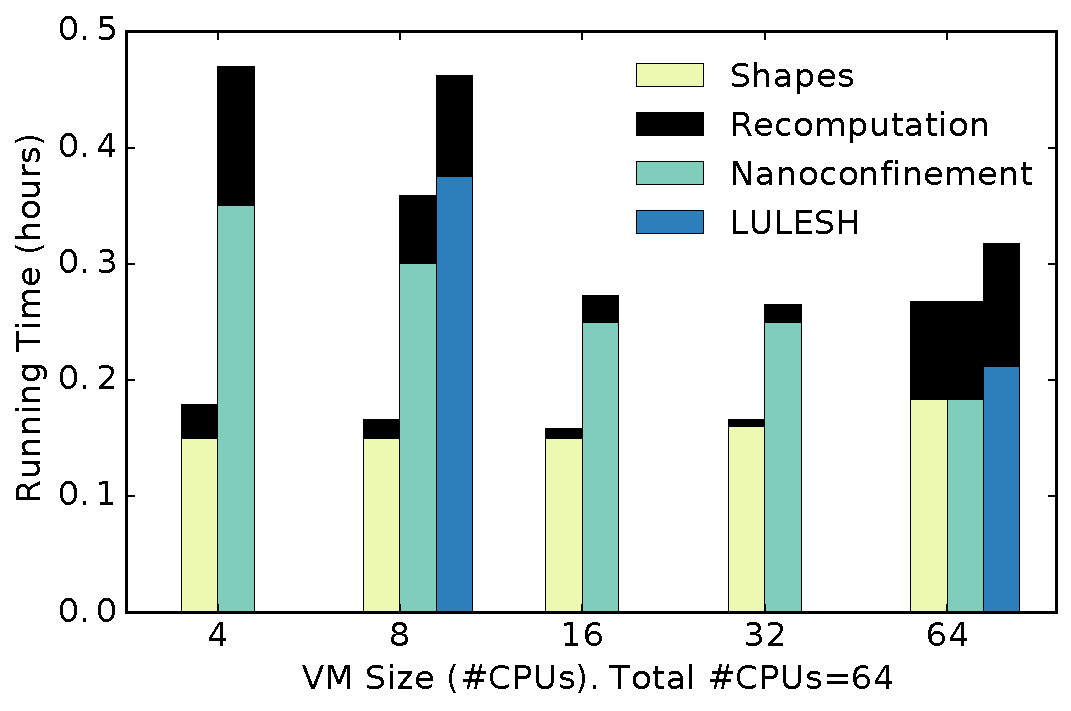
\includegraphics[width=0.4\textwidth]{../graphs/runtime-bars.pdf}
  \caption{Running times of applications on different servers}
  \label{fig:runtimes-bar}
\end{figure}

As described in Section~\ref{sec:design}, applications can be deployed on multiple types of VMs in the cloud, with each VM type having a different number of CPUs. 
Figure~\ref{fig:runtimes-bar} shows the running times of the different applications 

\noindent \emph{ \textbf{Result:} Running time is cluster configuration dependent, and increase in running time due to recomputation is small and less than 5\%.}



\begin{figure}
  \centering
  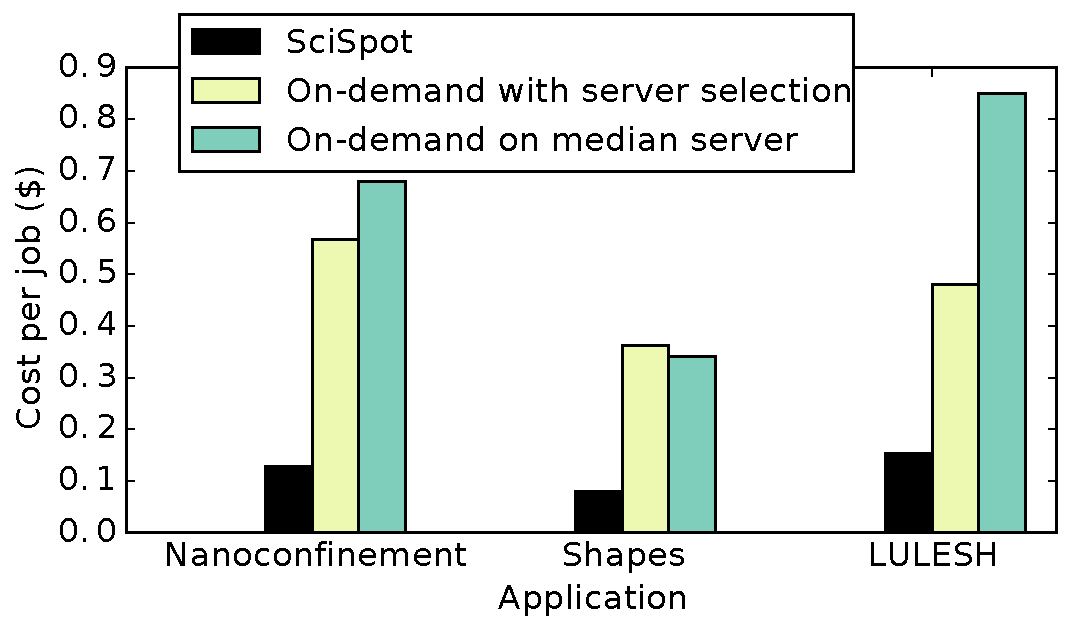
\includegraphics[width=0.4\textwidth]{../graphs/cost-only-bar.pdf}
  \caption{Cost of different configurations}
  \label{fig:cost-only-bar}
\end{figure}

\noindent \emph{ \textbf{Result:} SciSpot reduces computing costs by up to 5x and 7x compared to on-demand cloud servers.}

\begin{figure}
  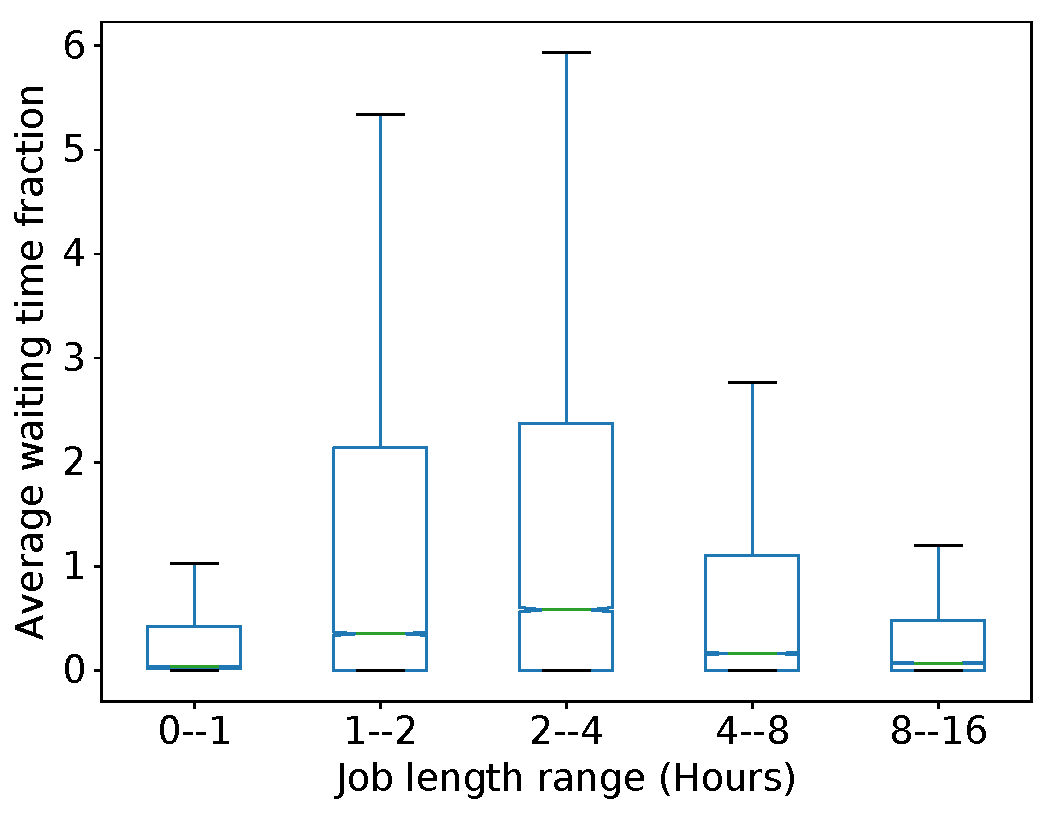
\includegraphics[width=0.4\textwidth]{../graphs/waiting_time_buckets.pdf}
  \caption{Waiting time fraction of jobs of different lengths varies.}
  \label{fig:hpc-wait-buckets}  
\end{figure}

\noindent \emph{ \textbf{Result:} While preemptions can increase running times due to recomputation, this increase is small, and is between 20 to 400\% lower compared to conventional HPC clusters. }

\subsection{Total cost vs. running time graphs}

\begin{figure}
  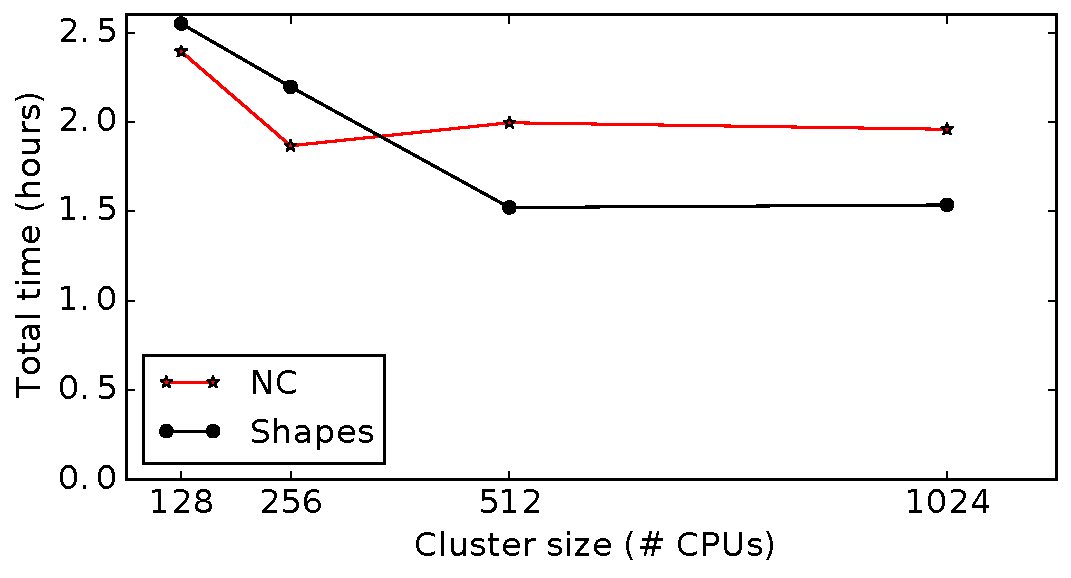
\includegraphics[width=0.2\textwidth]{../graphs/vm-per-job-scaling.pdf}
  \caption{SciSpot scaling as the VMs per jobs increases}
  \label{fig:vm-per-job-scaling}
\end{figure}

Figure~\ref{fig:vm-per-job-scaling} shows the total bag of job execution times for 32 jobs with 4 jobs running in parallel.
32 CPU VM's were used, and thus the total number of CPUs = 32*jobs-per-VM. Max CPU's used was 512 


\begin{figure}
  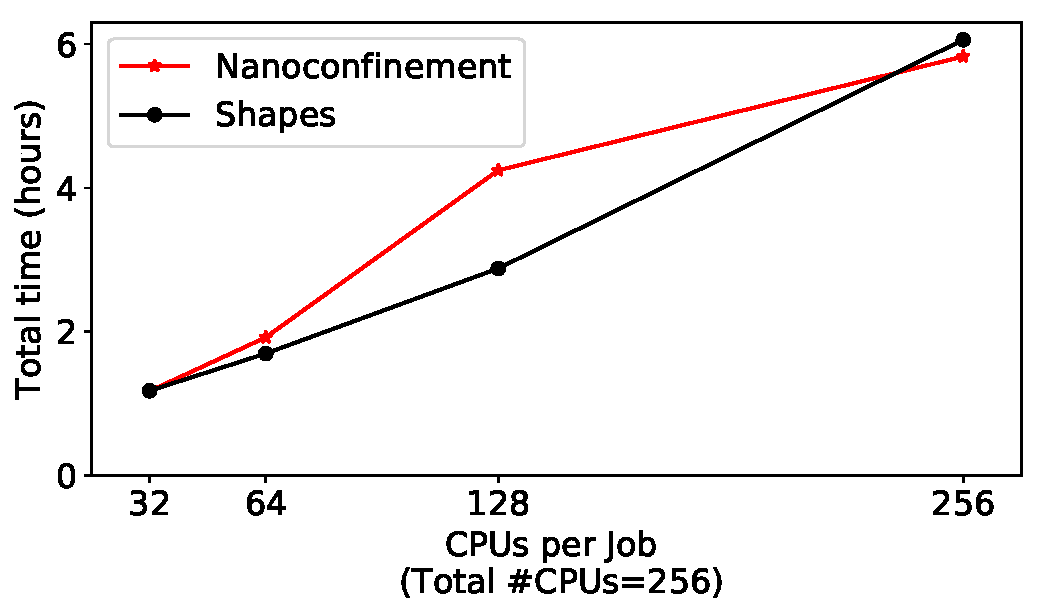
\includegraphics[width=0.2\textwidth]{../graphs/par-scaling.pdf}
  \caption{Job running times as the CPU's per job increases}
  \label{fig:par-scaling}
\end{figure}

Figure~\ref{fig:par-scaling} shows the running time when the total cluster size is fixed, but the number of parallel jobs and hence the number of CPUs per job changes. 



\subsection{Comparison with HPC Clusters}


% \begin{figure}
%   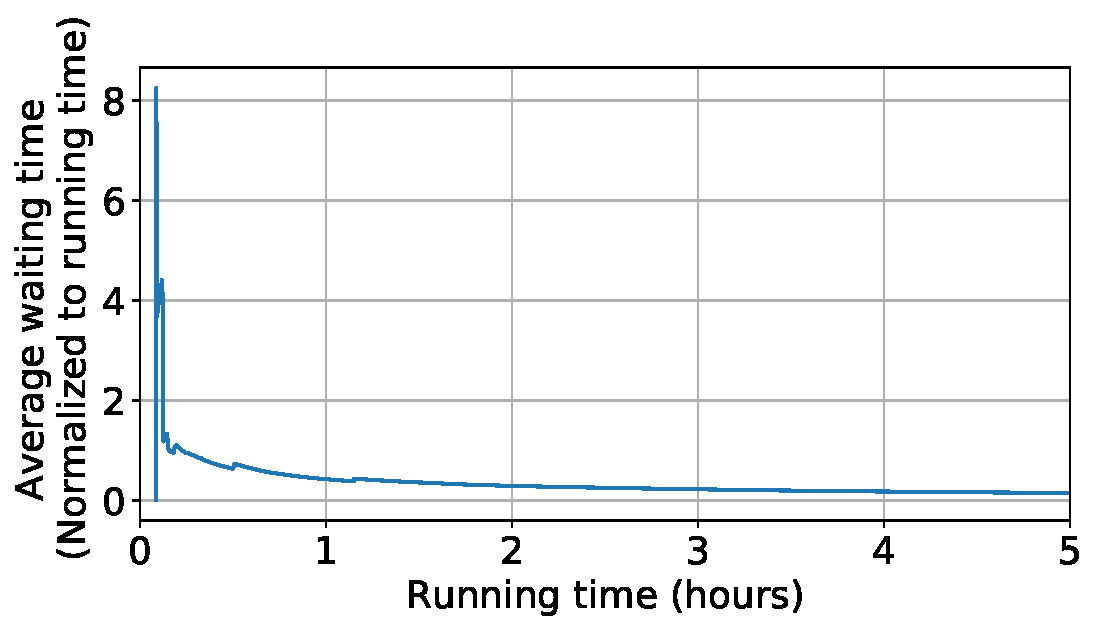
\includegraphics[width=0.4\textwidth]{../data/waiting_cumul.pdf}
%   \caption{The average waiting time (normalized to running time) of jobs of different length.}
%   \label{fig:hpc-wait-cdf}
% \end{figure}



%%% Local Variables:
%%% mode: latex
%%% TeX-master: "paper"
%%% End:
